\chapter{Метод обучения с подкреплением} \label{chapt1}
При постановке задач обучения с подкреплением (Reinforcement learning, коротко RL) исследуемую систему условно разделяют на два блока: агент и динамический процесс или среда. Агент - структурно автономная система, которая в процессе функционирования системы производит наблюдения, выбирает действие и применяет это действие на среду, меняя её состояние. Схематичная визуализация взаимодействия показана на рисунке \ref{img:rl} Цель агента - выбирать адекватные задаче действия.

\begin{figure}[ht] 
	\center
	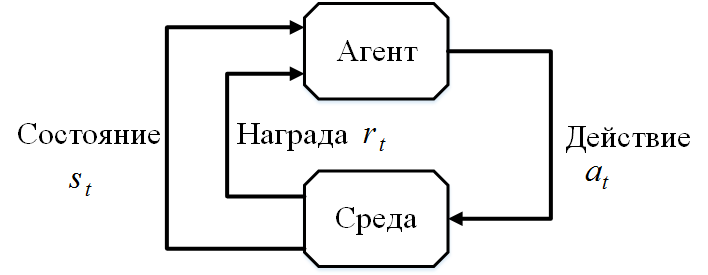
\includegraphics [scale=0.7] {rl}
	\caption{Схема взаимодействия агента со средой} 
	\label{img:rl}  
\end{figure}

В процессе обучения агент принимает специальный скалярный сигнал от среды - подкрепление. Этот сигнал показывает, насколько хорошо агент выполняет поставленную задачу. Обычно этот сигнал связывается только с теми событиями, которые кардинально влияют на процесс: успешное выполнение части задачи, задачи целиком (сигнал награды) или же наоборот, критическая ошибка агента (сигнал штрафа), приведшая к драматическим событиям. Именно этот аспект отличает обучение с подкреплением от обучения с учителем (supervised learning), при котором предоставляются пары "входные данные - ответ". 

\section{Постановка задачи управления с применением обучения с подкреплением} \label{sect1_1}

В произвольный момент времени $ t_i $ агент принимает состояние среды $ s_i\in S $, где $ S $ некоторое конечное множество возможных состояний внешней среды, и, базируясь на этой информации, вырабатывает определенное воздействие на среду $ a_i\in A(s_i) $, где $ A(s_i) $ конечное множество действий, которые могут быть оказаны на среду в состоянии $ s_i $. Данное воздействие $ a_i $ переводит среду в состояние $ s_{i+1} $, а агент получает вознаграждение $ r_i $. Агент в процессе обучения должен выработать такую стратегию $ \pi: S \rightarrow A $, чтобы максимизировать $ R_i $ - суммарную величину всех подкреплений.

Различают два типа задач обучения с подкреплением:
\begin{itemize}
	\item задачи с терминальным состоянием - эпизодические;
	\item задачи без терминального состояния - непрерывные.
\end{itemize}

Для эпизодической задачи $ R_i $ определяется как:
\begin{equation}
\label{eq:1_1p1}
\begin{alignedat}{2}
R_i=r_{i+1} + r_{i+2} + \cdots + r_N = \sum \limits_{k=i}^{N}r_{i+1+k} \end{alignedat}
\end{equation}
где $ i $ - номер шага, а $ N $ - количество шагов в эпизоде.

В отличии от эпизодических задач, где эпизод состоит из конечного числа шагов и суммарная величина подкрепления всегда может быть ограничена некоторой максимальной величиной, непрерывные задачи могут иметь $ R_i $ стремящееся к бесконечности. Для таких случаев применяют выражение:
Для эпизодической задачи $ R_i $ определяется как:
\begin{equation}
\label{eq:1_1p2}
\begin{alignedat}{2}
R_i=r_{i+1} + \gamma \cdot r_{i+2} + \gamma^2 \cdot r_{i+3} + \cdots = \sum \limits_{k=0}^{\infty}\gamma^k \cdot r_{i+1+k}
\end{alignedat}
\end{equation}
где $ \gamma \in [0, 1]$ - коэффициент дисконтирования подкрепления, который обеспечивает сходимость суммарной величины подкрепления.  
Параметр дисконтирования взвешивает значения подкрепления, полученные в прошлом относительно новых. Чем ближе $ \gamma $ к единице, тем больше агентом принимаются во внимание новые сигналы от среды, а если $ \gamma = 0 $, то все будущие сигналы подкрепления никак не будут учтены. 
%\newpage\S
%============================================================================================================================

\section{Функции оценки} \label{sect1_2}
Как уже было показано, обучение с подкреплением имеет дело с наградами и штрафами, которые принимаются от среды, но данные сигналы имеют сиюминутный характер и не могут прямо использоваться как данные о качестве работы агента. Практически все алгоритмы обучения с подкреплением используют функции оценки, которые бывают двух видов:
\begin{itemize}
	\item функция оценки состояния среды (value function);
	\item функция оценки воздействия агента на среду (Q-function).
\end{itemize}

Функция оценки состояния среды обозначается как $ V $ и связывает состояние среды $ s $ c её оценкой $ V(s) $. Для стратегии управления $ \pi $ оценка состояния среды $ s $ будет определятся как сумма всех подкреплений, которые получит агент в будущем следуя данной стратегии управлений:
 
$$ V^\pi(s)=R_i=\sum \limits_{k=0}^{\infty}\gamma^k \cdot r_{i+1+k}. $$

\noindent где $ s $ - состояние среды на текущем шаге($ s_i=s $), $ i $ - текущий шаг. 

$ V^\pi(s) $ можно выразить через оценку состояния среды и сигнал подкрепления на следующем шаге:

\begin{equation}
\label{eq:1_2p1}
\begin{alignedat}{2}
V^\pi(s)=r_{i+1} + \gamma\cdot\sum\limits_{k=0}^{\infty}\gamma^k \cdot r_{i+2+k}=r_{i+1} + \gamma \cdot V^\pi(s_{i+1}).
\end{alignedat}
\end{equation}

Функция оценки воздействия обозначается $ Q $ и связывает состояние среды $ s $ и воздействие $ a $ с оценкой воздействия $ Q(s,a) $. Для стратегии управления $ \pi $ оценка воздействия $ a $ при состоянии среды $ s $ определяется как сумма будущих подкреплений начиная с состояния $ s $ и если агент применит воздействие $ a $:

\begin{equation}
\label{eq:1_2p2}
\begin{alignedat}{2}
Q^\pi (s,a) = R_i = \sum\limits_{k=0}^{\infty}\gamma^k \cdot r_{i+1+k}.
\end{alignedat}
\end{equation}

\noindent где $ a $ - воздействие на шаге $ i $ ($ a=a_i $). Предполагается, что действие $ a $ на следующем шаге и далее будет удовлетворять стратегии $ \pi $, то есть $ a_k=\pi(s_k) $ для всех $ k=i+1, i+2, i+3, ... $ Оценка воздействия на текущем шаге выражается через оценку воздействия на следующем шаге и подкрепление на следующем шаге:

\begin{equation}
\label{eq:1_2p3}
\begin{alignedat}{2}
Q^\pi (s,a) = r_{i+1} + \gamma\cdot\sum\limits_{k=0}^{\infty}\gamma^k \cdot r_{i+2+k}=r_{i+1} + \gamma \cdot Q^\pi(s_{i+1}, \pi(s_{i+1})).
\end{alignedat}
\end{equation}

Функцию оценки состояния среды можно выразить через функцию оценки воздействия, зная при этом стратегию управления. Для этого необходимо для каждого состояния определить воздействие исходя из стратегии управления $ a_i = \pi(s_i) $:

\begin{equation}
\label{eq:1_2p4}
\begin{alignedat}{2}
V^\pi(s) = Q^\pi(s, \pi(s)).
\end{alignedat}
\end{equation}

Подставляя (\ref{eq:1_2p4}) в (\ref{eq:1_2p3}) получив формулу нахождения оценки воздействия на текущем шаге через оценку состояния на следующем:

\begin{equation}
\label{eq:1_2p5}
\begin{alignedat}{2}
Q^\pi(s, a) = r_{i+1} + \gamma\cdot V^\pi(s_{i+1}).
\end{alignedat}
\end{equation}

\section{Алгоритмы обучения} \label{sect1_3}

\subsection{Алгоритм временных разностей} \label{subsect1_3_1}

\subsection{Алгоритм SARSA} \label{subsect1_3_2}
SARSA (state-action-reward-state-action) алгоритм "состояние-действие-награда-состояние-действие" относят к классу динамического программирование с применением эвристик. 

\begin{equation}
\label{eq:1_3_2p1}
\begin{alignedat}{2}
Q(s_{t},a_{t}) \leftarrow Q(s_{t},a_{t}) + \alpha[r_{t} + \gamma Q(s_{t+1},a_{t+1}) - Q(s_{t},a_{t})], 0 \le \gamma \le 1.
\end{alignedat}
\end{equation}

\subsection{Алгоритм Q-обучения} \label{subsect1_3_3}

Q-обучение это алгоритм, в основе которого лежит отложенное  вознаграждение [Уоткинс 89]. Целью данного алгоритма является максимизация Q(s, a) – ожидаемого дисконтированного вознаграждения рассчитанного для действия а при состоянии s. Алгоритм рассчитывает и обновляет значения Q для каждой комбинации «состояние-действие»

\begin{equation}
\label{eq:1_3_3p1}
\begin{alignedat}{2}
s' \leftarrow T(s,a),\\
E(s)=max_{a}Q(s,a),\\
Q(s,a)=r + \gamma(E(s')).
\end{alignedat}
\end{equation}

Q расчитывается по следующему правилу:

\begin{equation}
\label{eq:1_3_3p2}
\begin{alignedat}{2}
Q(s,a) \leftarrow Q(s,a) + \beta(r + \gamma E(s') - Q(s,a)), 0 \le \gamma \le 1.
\end{alignedat}
\end{equation}

\subsection{Глубокое Q-обучения} \label{subsect1_3_4}

\subsection{Алгоритм $TD(\lambda)$} \label{subsect1_3_5}

\subsection{Метод Актор-Критик} \label{subsect1_3_6}

\begin{figure}[ht] 
	\center
	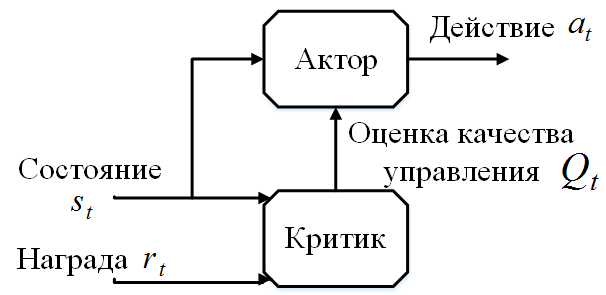
\includegraphics [scale=0.7] {ac}
	\caption{Структурная схема Актор-Критик метода} 
	\label{img:ac}  
\end{figure}

\subsection{Анализ алгоритмов обучения} \label{subsect1_3_7}

